\documentclass[11pt]{beamer}

\usetheme{Madrid}
\setbeamertemplate{navigation symbols}{}

% Math and graphics
\usepackage{amsmath,amssymb,amsthm,mathtools,bm}
\usepackage{graphicx}
\graphicspath{{images/}}
\usepackage{pgfplots}
\pgfplotsset{compat=1.18}
\usepackage{tikz}
\usetikzlibrary{arrows.meta,calc,decorations.markings}
\usepackage{tikz-cd}
\usepackage[most]{tcolorbox}
\usepackage{hyperref}
\usepackage{csquotes}
\usepackage{cancel}

% If you really have Kyushu.sty installed, uncomment this.
% \usepackage{Kyushu}

% Theorem-like environments
\theoremstyle{definition}
\newtheorem{exercise}{Exercise}[section]

\theoremstyle{plain}
\newtheorem{conjecture}{Conjecture}[section]

% Short macros
\newcommand{\C}{\mathbb{C}}
\newcommand{\R}{\mathbb{R}}
\newcommand{\Arg}{\operatorname{Arg}}
\newcommand{\card}{\operatorname{card}}

\title[MAT215]{MAT215: Complex Variables and Laplace Transformations}
\author[Emon Hossain]{Emon Hossain}
\institute[University of Dhaka]{Lecturer\\MNS Department\\BRAC University}
\date{Lecture 06}

\AtBeginSection[]
{
  \begin{frame}{Table of Contents}
    \tableofcontents[currentsection]
  \end{frame}
}

\begin{document}

\begin{frame}
\titlepage
\end{frame}

%------------------------------------------------
\section{Visualizing Complex Functions}

\begin{frame}{Intuition}
If you want to study a space, it is often helpful to study how functions behave on that space.

When we view \(\C\) as \(\R^2\) with extra structure, a complex-valued function
\[
f:\C\to\C,\qquad z\mapsto w=f(z)
\]
has both input and output in two real dimensions.

So the pair \((z,f(z))\) really lives in \(4\) real dimensions:
\[
(z,f(z))=(x,y,u,v).
\]

That is why visualizing complex functions needs some clever tricks.
\end{frame}

\begin{frame}{Ways to Visualize Complex Functions}
There are several common ways to visualize complex functions:
\begin{itemize}
    \item Domain coloring
    \item \(3D\) plots
    \item Vector fields
    \item \(z\)-\(w\) planes
    \item Riemann sphere
\end{itemize}

In domain coloring, the output \(f(z)\) is represented by color:
\[
\text{Hue}\leftrightarrow\text{Argument},
\qquad
\text{Lightness}\leftrightarrow\text{Modulus}.
\]
\end{frame}

\begin{frame}{\(3D\) Plots}
In a \(3D\) plot, we sacrifice one real variable from
\[
(z,f(z))=(x,y,u,v)
\]
and represent the missing variable by color.

For example:
\[
\text{missing }v \leftrightarrow \text{color}.
\]
For more details: \url{https://www.youtube.com/watch?v=NtoIXhUgqSk}.
\end{frame}

\begin{frame}{Multi-Valued Functions and Branches}
\begin{definition}
A multi-valued function \(f\) on \(E\subset \C\) assigns a set of complex values to each \(z\in E\). In other words, \(f(z)\) is a set of complex numbers.
\end{definition}

\begin{definition}
A branch of a multi-valued function \(f\) on \(E\subset \C\) is a single-valued function obtained by choosing one value from \(f(z)\) for each \(z\in E\).
\end{definition}
\end{frame}

\begin{frame}{A Complex Function as Two Real Functions}
For a function
\[
f:D\subseteq\C\to\C,
\]
write
\[
z=x+iy,\qquad w=f(z)=u+iv.
\]

Then
\[
w=f(x+iy)=u(x,y)+iv(x,y).
\]

So instead of studying one complex function, we can study two real-valued functions:
\[
u(x,y)\quad\text{and}\quad v(x,y).
\]
\end{frame}

\begin{frame}{Polar Point of View}
If
\[
z=re^{i\theta},
\]
then the output can also be written as
\[
w=f(z)=f(re^{i\theta})=u(r,\theta)+iv(r,\theta).
\]

Sometimes rectangular coordinates are more convenient, and sometimes polar coordinates are better.

This depends on the function we are studying.
\end{frame}

%------------------------------------------------
\section{The Complex Exponential}

\begin{frame}{Complex Exponential}
The exponential function is
\[
\exp:\C\to\C\setminus\{0\},
\]
defined by
\[
\exp(z)=\exp(x+iy)=e^x e^{iy}.
\]

Using Euler's formula,
\[
e^{iy}=\cos y+i\sin y,
\]
we get
\[
\exp(x+iy)=e^x(\cos y+i\sin y).
\]
\end{frame}

\begin{frame}{Modulus and Argument of \(e^z\)}
From
\[
\exp(x+iy)=e^x e^{iy},
\]
we immediately obtain:
\[
\left|\exp(x+iy)\right|=e^x,
\qquad
\arg(\exp(x+iy))=y+2\pi\mathbb{Z}.
\]

So:
\begin{itemize}
    \item the real part \(x\) controls the modulus,
    \item the imaginary part \(y\) controls the argument.
\end{itemize}
\end{frame}

\begin{frame}{Why Is the Exponential Map a Homomorphism?}
For \(z_1,z_2\in\C\),
\[
e^{z_1+z_2}=e^{z_1}e^{z_2}.
\]

So the exponential map is a homomorphism from the additive group \((\C,+)\) to the multiplicative group \((\C\setminus\{0\},\cdot)\).

Its kernel is
\[
\ker(\exp)=2\pi i\,\mathbb{Z}.
\]

Hence it induces
\[
\exp:\bigl(\C/(2\pi i\,\mathbb Z),+\bigr)\to(\C\setminus\{0\},\cdot).
\]

\begin{tcolorbox}
The period is in the imaginary direction, so the quotient must be by \(2\pi i\,\mathbb Z\), not by \(2\pi\mathbb Z\).
\end{tcolorbox}
\end{frame}

\begin{frame}{Horizontal Lines Under \(w=e^z\)}
\begin{columns}[T,onlytextwidth]
\column{0.48\textwidth}
\centering
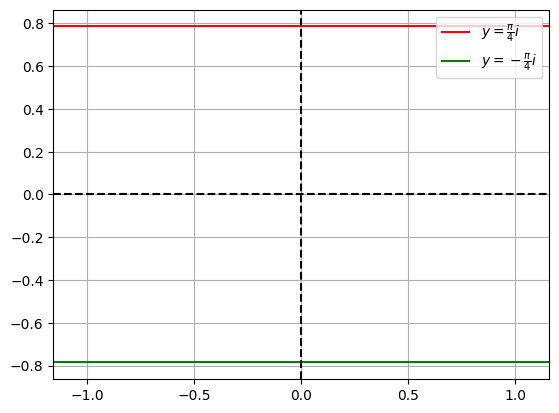
\includegraphics[width=\linewidth,height=0.48\textheight,keepaspectratio]{exp z horizontal lines.png}

\small Input: \(z=x\pm \frac{\pi}{4}i\)

\column{0.48\textwidth}
\centering
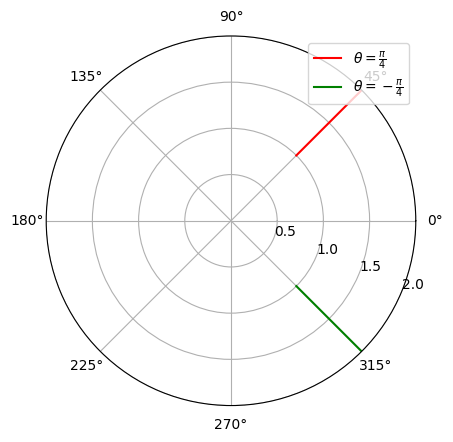
\includegraphics[width=\linewidth,height=0.48\textheight,keepaspectratio]{exp z horizontal lines out.png}

\small Output: \(r=e^x,\ \theta=\pm \frac{\pi}{4}\)
\end{columns}
\end{frame}

\begin{frame}{Horizontal Lines Become Rays}
For the line
\[
z=x+\frac{\pi}{4}i,
\]
we get
\[
\exp(z)=\exp\!\left(x+\frac{\pi}{4}i\right)=e^x e^{i\pi/4}.
\]

Comparing with polar form:
\[
r=e^x,\qquad \theta=\frac{\pi}{4}.
\]

So the image is a ray making angle \(\frac{\pi}{4}\) with the positive real axis.

Similarly,
\[
z=x-\frac{\pi}{4}i
\quad\Longrightarrow\quad
\exp(z)=e^x e^{-i\pi/4},
\]
which is the ray at angle \(-\frac{\pi}{4}\).
\end{frame}

\begin{frame}{Why Does the Ray Not Include the Origin?}
For
\[
\exp(z)=e^x e^{i\theta},
\]
the modulus is
\[
r=e^x.
\]

But \(e^x>0\) for every real \(x\), so the modulus can get arbitrarily small, but it can never be \(0\).

That is why the image ray approaches the origin but never actually reaches it.
\end{frame}

\begin{frame}{Vertical Lines Under \(w=e^z\)}
\begin{columns}[T,onlytextwidth]
\column{0.48\textwidth}
\centering
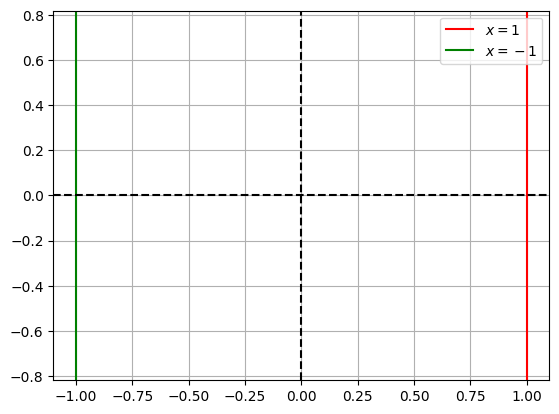
\includegraphics[width=\linewidth,height=0.48\textheight,keepaspectratio]{exp z vertical lines.png}

\small Input: \(z=\pm 1+iy\)

\column{0.48\textwidth}
\centering
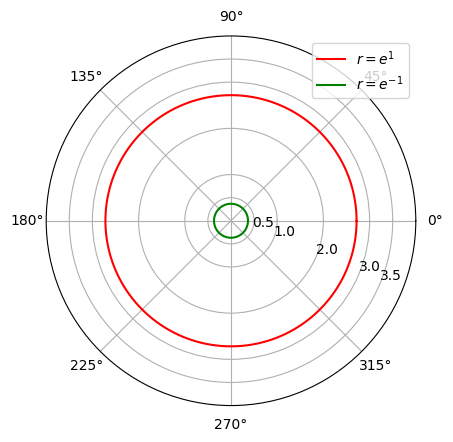
\includegraphics[width=\linewidth,height=0.48\textheight,keepaspectratio]{exp z vertical lines out.png}

\small Output: \(r=e^{\pm1}\)
\end{columns}
\end{frame}

\begin{frame}{Vertical Lines Become Circles}
Take
\[
z=1+iy.
\]
Then
\[
\exp(z)=\exp(1+iy)=e^1 e^{iy}.
\]

So
\[
r=e,\qquad \theta=y.
\]

Since \(y\) varies, the angle varies while the radius stays fixed. Therefore the image is the circle of radius \(e\).

Likewise,
\[
z=-1+iy
\]
maps to the circle of radius \(e^{-1}\).
\end{frame}

\begin{frame}{A Vertical Strip Under \(w=e^z\)}
\begin{columns}[T,onlytextwidth]
\column{0.48\textwidth}
\centering
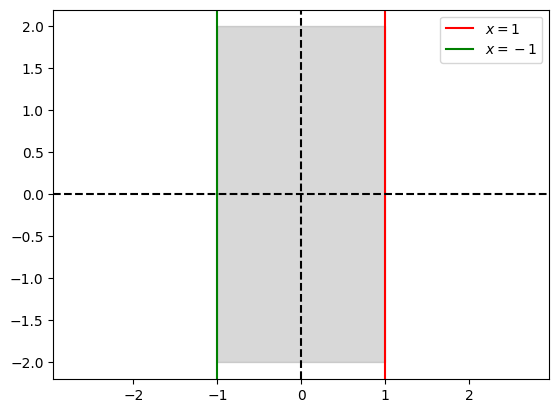
\includegraphics[width=\linewidth,height=0.48\textheight,keepaspectratio]{exp z vertical strip.png}

\small Input strip: \(-1\le \Re(z)\le 1\)

\column{0.48\textwidth}
\centering
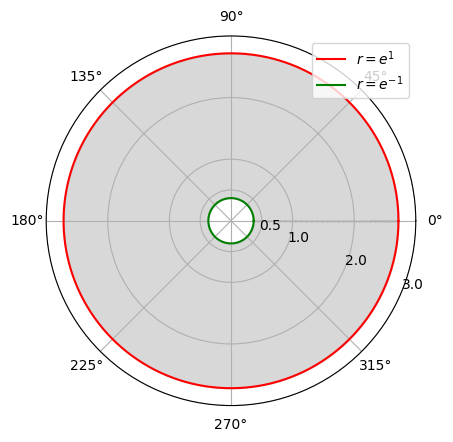
\includegraphics[width=\linewidth,height=0.48\textheight,keepaspectratio]{exp z vertical strip out.png}

\small Output annulus: \(e^{-1}\le |w|\le e\)
\end{columns}
\end{frame}

\begin{frame}{Vertical Strip Becomes an Annulus}
Let
\[
z=x+iy,\qquad -1\le x\le 1.
\]

Under \(w=e^z\),
\[
|w|=e^x.
\]

So:
\[
x=1 \Longrightarrow |w|=e,
\qquad
x=-1 \Longrightarrow |w|=e^{-1}.
\]

Hence
\[
e^{-1}\le |w|\le e.
\]

Since \(y\) is free, the argument runs through all angles, so the strip maps onto the annulus bounded by
\[
|w|=e^{-1}
\quad\text{and}\quad
|w|=e.
\]
\end{frame}

\begin{frame}{Exercise}
\begin{exercise}
Find the image of the horizontal strip in the \(z\)-plane lying between
\[
z=x+\frac{\pi}{4}i
\qquad\text{and}\qquad
z=x-\frac{\pi}{4}i
\]
under the map \(w=e^z\).
\end{exercise}
\end{frame}

%------------------------------------------------
\subsection{Complex Powers}

\begin{frame}{Complex Powers}
With the logarithm, we can define complex powers.

Let \(\alpha\in\C\). For \(z\neq 0\), define
\[
z^\alpha \equiv e^{\alpha \log z}.
\]

Using \(\log z=\log|z|+i\arg(z)\), this becomes
\[
z^\alpha = e^{\alpha \log|z|+i\alpha \arg(z)}.
\]

Because \(\arg(z)\) is multi-valued, \(z^\alpha\) is generally multi-valued as well.
\end{frame}

\begin{frame}{Why Complex Powers Are Multi-Valued}
Write
\[
\arg(z)=\Arg(z)+2\pi k,\qquad k\in\mathbb Z.
\]

Then
\[
z^\alpha
= e^{\alpha \log|z|+i\alpha(\Arg(z)+2\pi k)}
= e^{\alpha \log|z|+i\alpha\Arg(z)}\,e^{i2\pi\alpha k}.
\]

So different integers \(k\) may produce different values.

Depending on \(\alpha\), the function may have:
\begin{itemize}
    \item one value,
    \item finitely many values,
    \item infinitely many values.
\end{itemize}
\end{frame}

\begin{frame}{Exercise}
\begin{exercise}
Find all possible values of \(i^i\) and \(1^i\).
\end{exercise}
\end{frame}

%------------------------------------------------
\section{Complex Trigonometric Functions}

\begin{frame}{Hyperbolic Functions First}
Recall:
\[
\sinh x=\frac{e^x-e^{-x}}{2},
\qquad
\cosh x=\frac{e^x+e^{-x}}{2},
\qquad
\tanh x=\frac{e^x-e^{-x}}{e^x+e^{-x}}.
\]

Now plug in purely imaginary numbers into the trigonometric formulas.
\end{frame}

\begin{frame}{Trigonometric--Hyperbolic Identities}
We compute:
\[
\cos(ix)=\frac{e^{i(ix)}+e^{-i(ix)}}{2}
=\frac{e^{-x}+e^x}{2}
=\cosh x.
\]

Similarly,
\[
\sin(ix)=i\sinh x,
\qquad
\tan(ix)=i\tanh x.
\]
\end{frame}

\begin{frame}{Formula for \(\sin(x+iy)\)}
Using angle addition,
\[
\sin(x+iy)=\sin x\cos(iy)+\cos x\sin(iy).
\]

Now use
\[
\cos(iy)=\cosh y,
\qquad
\sin(iy)=i\sinh y.
\]

Therefore,
\[
\sin(x+iy)=\sin x\cosh y+i\cos x\sinh y.
\]
\end{frame}

\begin{frame}{Formula for \(\cos(x+iy)\)}
Similarly,
\[
\cos(x+iy)=\cos x\cos(iy)-\sin x\sin(iy).
\]

Hence,
\[
\cos(x+iy)=\cos x\cosh y-i\sin x\sinh y.
\]
\end{frame}
\begin{frame}{Inverse Circular Functions}
  The inverse circular functions for complex numbers are defined as follows:

\[
\sin^{-1} z = -i \ln \left( iz + \sqrt{1 - z^2} \right)
\]

\[
\cos^{-1} z = -i \ln \left( z + \sqrt{z^2 - 1} \right)
\]

\[
\tan^{-1} z = \frac{i}{2} \ln \left( \frac{i + z}{i - z} \right)
\]

\[
\cot^{-1} z = \frac{i}{2} \ln \left( \frac{z - i}{z + i} \right)
\]

\[
\sec^{-1} z = -i \ln \left( \frac{1 + \sqrt{1 - z^2}}{z} \right)
\]

\[
\csc^{-1} z = -i \ln \left( \frac{i + \sqrt{z^2 - 1}}{z} \right)
\]
\end{frame}
\begin{frame}
  show that, \[
\tan^{-1} z = \frac{i}{2} \ln \left( \frac{i + z}{i - z} \right)
\]

  \[
\text{Let } \theta=\tan^{-1}z
\quad\Rightarrow\quad
z=\tan\theta
\]

\[
\Rightarrow z=\frac{\sin\theta}{\cos\theta}
\]

\[
\Rightarrow z=
\frac{\dfrac{e^{i\theta}-e^{-i\theta}}{2i}}
{\dfrac{e^{i\theta}+e^{-i\theta}}{2}}
\]

\[
\Rightarrow z=
\frac{e^{i\theta}-e^{-i\theta}}
{i\left(e^{i\theta}+e^{-i\theta}\right)}
\]

\[
\Rightarrow iz=
\frac{e^{i\theta}-e^{-i\theta}}
{e^{i\theta}+e^{-i\theta}}
\]
\end{frame}
\begin{frame}
By componendo and dividendo,
\[
\frac{1+iz}{1-iz}
=
\frac{(e^{i\theta}-e^{-i\theta})+(e^{i\theta}+e^{-i\theta})}
{(e^{i\theta}+e^{-i\theta})-(e^{i\theta}-e^{-i\theta})}
\]
  \[
\Rightarrow
\frac{1+iz}{1-iz}
=
\frac{2e^{i\theta}}{2e^{-i\theta}}
\]

\[
\Rightarrow
\frac{1+iz}{1-iz}=e^{2i\theta}
\]

\[
\Rightarrow
2i\theta=\ln\left(\frac{1+iz}{1-iz}\right)
\]

\[
\Rightarrow
\theta=\frac{1}{2i}\ln\left(\frac{1+iz}{1-iz}\right)
\]

Since \(\dfrac{1}{i}=-i\),
\[
\theta=-\frac{i}{2}\ln\left(\frac{1+iz}{1-iz}\right)
\]
\end{frame}
\begin{frame}
Now,
\[
1+iz=i(z-i),\qquad 1-iz=-i(z+i)
\]
So,
\[
\frac{1+iz}{1-iz}
=
\frac{i(z-i)}{-i(z+i)}
=
-\frac{z-i}{z+i}
=
\frac{i-z}{i+z}
\]

Hence,
\[
-\frac{i}{2}\ln\left(\frac{1+iz}{1-iz}\right)
=-\frac{i}{2}\ln\left(\frac{i-z}{i+z}\right)
= \frac{i}{2}\ln\left(\frac{i+z}{i-z}\right)
\]

Therefore,
\[
\boxed{
\tan^{-1}z=\frac{i}{2}\ln\left(\frac{i+z}{i-z}\right)
}
\]
\end{frame}
\begin{frame}{Inverse Hyperbolic Functions}
The inverse hyperbolic functions for complex numbers are defined as follows:
\[
\sinh^{-1} z = \ln\left( z + \sqrt{z^2 + 1} \right)
\]

\[
\cosh^{-1} z = \ln\left( z + \sqrt{z^2 - 1} \right)
\]

\[
\tanh^{-1} z = \frac{1}{2}\ln\left( \frac{1+z}{1-z} \right)
\]

\[
\coth^{-1} z = \frac{1}{2}\ln\left( \frac{z+1}{z-1} \right)
\]

\[
\operatorname{sech}^{-1} z = \ln\left( \frac{1+\sqrt{1-z^2}}{z} \right)
\]

\[
\operatorname{cosech}^{-1} z = \ln\left( \frac{1+\sqrt{1+z^2}}{z} \right)
\]
\end{frame}
\end{document}